% Created 2022-05-12 Чт 10:09
% Intended LaTeX compiler: xelatex
\documentclass[11pt]{article}
\usepackage{graphicx}
\usepackage{longtable}
\usepackage{wrapfig}
\usepackage{rotating}
\usepackage[normalem]{ulem}
\usepackage{amsmath}
\usepackage{amssymb}
\usepackage{capt-of}
\usepackage{hyperref}
\usepackage[utf8x]{inputenc}
% \usepackage[T2A]{fontenc}

\usepackage[russian, english]{babel}
\babelfont{rm}{Droid Serif}
\babelfont{sf}{Droid Sans}
\babelfont{tt}{Droid Sans Mono Slashed}

\hypersetup{colorlinks=true,linkcolor=blue}

\let\oldsection\section
\renewcommand\section{\pagebreak\oldsection}

\usepackage{siunitx}
\sisetup{per-mode=symbol}

% \usepackage{minted}

\author{Андрей Люнгрин Иван Наумов}
\date{11 Мая 2022}
\title{Инженеры будущего\\\medskip
\large Rescue line}
\hypersetup{
 pdfauthor={Андрей Люнгрин Иван Наумов},
 pdftitle={Инженеры будущего},
 pdfkeywords={},
 pdfsubject={},
 pdfcreator={Emacs 28.1 (Org mode 9.6)}, 
 pdflang={English}}
\begin{document}

\maketitle
\tableofcontents


\section{Введение}
\label{sec:org70dcdc0}
Наша работа представляет из себя исследовательский проект проводимый в рамках соревнований под регламентов \texttt{RoboCup Junior RescueLine}. В рамках данной работы нами было разработано несколько прототипов роботизированных систем о которых пойдёт речь далее.
\section{Команда}
\label{sec:org037a8cb}
\subsection{Андрей Люнгрин}
\label{sec:orga33dff3}
\begin{center}

\includegraphics[width=100]{./images/andrey.jpeg}
\end{center}
\begin{itemize}
\item Капитан команды
\item Обязанности:
\begin{itemize}
\item Консультация по вопросам конструкции
\item Производство некоторых деталей
\item Финальная сборка и тестирование конструкции
\item Проектирование концепта
\item Разработка программных компонентов низкого уровня для управления приводами
\item Разработка программных компонентов для обеспечения связи между системами управления приводами и принятия решений
\item Разработка программной системы принятия решений
\item Сборка электронной составляющей робота
\item И просто хороший человек
\end{itemize}
\end{itemize}
\pagebreak
\subsection{Иван Наумов}
\label{sec:org96c6bcf}
\begin{center}
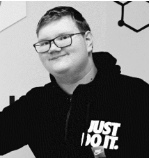
\includegraphics[width=100]{./images/ivan.jpg}
\end{center}
\begin{itemize}
\item Инженер-конструктор
\item Обязанности:
\begin{itemize}
\item Проектирование концепта
\item Моделирование конструкции робота в САПР
\item Производство основных деталей конструкци
\item Сборка конструкции
\end{itemize}
\end{itemize}
\section{Механическая часть}
\label{sec:org7fadcaf}
Основными целями при проектированнии конструкции были простоата и удобство обслуживания, и все последующие технические решения были направлены на улучшение этих двух метрик.

Все узлы робота были произведены с исопльзованием трёхмерной печати
\subsection{Колёсная платформа}
\label{sec:org92a5b89}
Конструктивно, робот представляет их себя четырёхколёсную тележку с двумя ведущими и двумя опорными колёмами. Опорные колеса были модифицированы так, чтобы максимально уменьшить сцепление с поверхностью. Это необходимо для того, чтобы кинематическая схема робота была приближена к таковой у двухколесного робота. Плюс такой схемы заключается в том, что ось поворота робота более предсказуема, и в меньшей степени зависит от распределения массы.

Каждое колесо имеет две точки опоры, что позволяет снизить изламывающие нагрузки на ось колеса, что увеличивает надёжность конструкции, а также делает положение колеса относительно рамы робота более предсказуемым.
\pagebreak
\subsection{Система захвата}
\label{sec:orgc0873ad}
Для захвата и сброса шариков и других игровых предметов, используется двух-осевой манипулятор. Первая ось обеспечивет подъём за счёт поворота всей сборки захвата. Вторая ось является клешнёй, которая выполняет захват объекта. Основное достоинство такой конструкции - её просто. Из недостатков, можно отметить её низкую точность позиционирования, и необходимость приложения высокого усилия мотором подъёма.
\subsection{Крепление электроники}
\label{sec:org73f232a}
Вся электронника робота закреплена на одной съёмной пластине, расположенной перпендикулярно плоскости рамы. Две основных платы раположены с разных сторон пластины. Такая конфигурация обеспечивает полный доступ ко всем элементам системы, а также позволяет быстро их демонтировать для замены или другого обслуживания.
\section{Электронная часть}
\label{sec:org15bf3c2}
Наша система состоит из трёх основных узлов:
\begin{enumerate}
\item Узел питания
\begin{itemize}
\item Распределяет питание из одного источника между всеми потребителями
\item Согласовывает питающие уровни
\item Состоит из:
\begin{itemize}
\item Высокотоковый литий-полимерный аккумулятор на 12V
\item Понижающий преобразователь
\item Соединительные колодки \texttt{Wago}
\end{itemize}
\end{itemize}
\item Узел принятия решений
\begin{itemize}
\item Получает и обрабатывает информацию об окружающем мире
\item Состоит из:
\begin{itemize}
\item Одноплатный компьютер: \texttt{Raspberry Pi 3B}
\item Основная передняя камера, для следования по линии: \texttt{Pi Camera}
\item Задняя камера для захвата предметов
\end{itemize}
\end{itemize}
\item Исполнительный узел
\begin{itemize}
\item Управляет шаговыми двигателями в ответ на команды с Узла принятия решений
\item Состоит из:
\begin{itemize}
\item Микроконтроллер на отладочной плате: \texttt{STN32 Nucleo-F401RE}
\item Материнская плата драйверов ШД: \texttt{Arduino CNC shield v3}
\item Четыре драйвера ШД: \texttt{StepStick A4988}
\item Два приводных шаговых двигателя
\item Два шаговых двигателя для манипулятора
\end{itemize}
\end{itemize}
\end{enumerate}

Шаговые двигатели для привода были использованы потому, что такой тип двигателя позволяет просто контроллировать их скорость, также тем, что существует множество готовых аппаратных решений для их управления. Простота управления и цена - вероятно единственные приимещества шаговых двигателей. К их недостаткам относятся: низкий КПД, низкое соотношение крутящего к массе двигателя, сильные вибрации. К счастью, все эти приблемы не значительны в нашем случае (нету ограничения по весу, низкие требования к тяге и времени автономной работы, а критерий простоты управления хорошо соотносится с целями проекта.

Решение использовать отдельный контроллер для управления двигателями были обосновано тем, что реализовать генерацию управляющих пульсов для драйверов ШД с микросекундной точностью, проще на системе реального времени, работая на низком уровне. Однако, такой подход влечет за собой усложнение системы, из-за необходимости обеспечивать связь между двумя контроллерами. В будущем, второй контроллер может быть упразднён.

\begin{center}
\includegraphics[width=.9\linewidth]{dot_success.png}
\end{center}
\end{document}
